% This is a draft of the coming paper "Multiple Round Ballot Polling Risk-Limiting Audit Simulations".
% 2021.
%
\documentclass[runningheads]{llncs}
%
\usepackage{float}
\usepackage{xspace}
\usepackage{graphicx}
\graphicspath{{./imgs/}}
\usepackage{comment}
\usepackage{listings,hyperref}
\usepackage{cite}

% \usepackage{graphicx}  --> Used for displaying a sample figure. If possible, figure files should
% be included in EPS format.
%
% If you use the hyperref package, please uncomment the following line
% to display URLs in blue roman font according to Springer's eBook style:
% \renewcommand\UrlFont{\color{blue}\rmfamily}


% nice looking audit titles
\newcommand{\Minerva}{\textsc{Minerva}\xspace}
\newcommand{\B}{{{B2}}\xspace}
\newcommand{\R}{{{R2}}\xspace}
\newcommand{\BRAVO}{\textsc{Bravo}\xspace}

\usepackage{color}
\definecolor{green}{rgb}{0.31, 0.78, 0.47}
\newcommand{\fpo}[1]{\textcolor{green}{#1}}

\def\code#1{\texttt{#1}}

\begin{document}
\lstset{language=Python}
%
\title{Simulations of Ballot Polling Risk-Limiting Audits}
%add \thanks{} within the title brackets if want to refer to supporting organization ^^
%
%\titlerunning{Abbreviated paper title}
% If the paper title is too long for the running head, you can set
% an abbreviated paper title here
%
\author{Oliver Broadrick\inst{1} \and
Sarah Morin\inst{1} \and
Grant McClearn\inst{2} \and Neal McBurnett \and Poorvi L. Vora\inst{1} \and
Filip Zag{\'o}rski\inst{3}\inst{4}}
%
\authorrunning{Broadrick, Morin et al.}
% First names are abbreviated in the running head.
% If there are more than two authors, 'et al.' is used.
%
\institute{Department of Computer Science, The George Washington University\thanks{Supported in part by NSF Award 2015253} 
\email{odbroadrick@gmail.com}\\
\and
Department of Computer Science, Stanford University 
\email{grantmcc@stanford.edu}
\\
\and Wroclaw University of Science and Technology\thanks{Author was partially supported by Polish National Science Centre contract number DEC-2013/09/D/ST6/03927} and 
\and Votifica
\\
\email{filip.zagorski@gmail.com}
}
%

\maketitle              % typeset the header of the contribution
%
\begin{abstract}
    In this paper we present simulation results comparing the risk, stopping probability, and number of ballots required over multiple rounds of ballot polling risk-limiting audits (RLAs) \Minerva, Selection-Ordered (SO) \BRAVO, and End-of-Round (EoR) \BRAVO.    
    \BRAVO is the most commonly used ballot polling RLA and requires the smallest expected number of ballots when ballots are drawn one at a time and the (true) underlying election is as announced. 
    In real audits, multiple ballots are drawn at a time, and \BRAVO is implemented as SO \BRAVO or EoR \BRAVO. 
    \Minerva is a recently proposed ballot polling RLA that requires fewer ballots than either implementation of \BRAVO in a first round with stopping probability $0.9$ but requires a predetermined round schedule.
    %\BRAVO is the most commonly used ballot polling RLA and requires the smallest expected number of ballots when ballots are drawn one at a time and the (true) underlying election is as announced. In real audits, election officials draw multiple ballots at a time, and \BRAVO rules may be implemented as SO \BRAVO or EoR \BRAVO, with neither being optimal for large first round sizes. \Minerva was recently proposed for use when the first-round stopping probability is large. It requires fewer first-round ballots, on average, than both SO \BRAVO and EoR \BRAVO for first round stopping probabilities of $0.9$ when the (true) underlying election is as announced. 
    It is an open question how these audits compare over multiple rounds and for lower stopping probabilities. 
    Our simulations use stopping probabilities of $0.9$ and $0.25$.
    %In this paper, we present results from simulations of multiple round audits with stopping probabilities of $0.9$ and $0.25$.
    %We examine both: first-round stopping probabilities of $0.9$, a common choice among election officials, and $0.25$, which would be more favorable to \BRAVO. 
    The results are consistent with predictions of the R2B2 open-source library for ballot polling audits. 
    %Because the \Minerva round schedule needs to be predetermined, we observe that the simulator is useful as a tool for understanding the behavior of \Minerva with the fixed round schedule. 
    We observe that both \BRAVO audits are more conservative than \Minerva, which stops with fewer ballots, for both first round stopping probabilities. 
    However, the advantage of using \Minerva decreases considerably for the smaller first round stopping probability, as one would expect. 

\keywords{risk-limiting audit (RLA)  \and ballot polling audit \and evidence-based elections \and statistical election audit}
\end{abstract}
%
%
\section{Introduction}
\label{sec:intro}
%Intro
The literature contains numerous descriptions of vulnerabilities in deployed voting systems, and it is not possible to be certain that any system, however well-designed, will perform as expected in all instances. For this reason, 
{\em evidence-based elections} \cite{evidence-based} aim to produce trustworthy and compelling evidence of the correctness of election outcomes, enabling the detection of problems with high probability. One way to implement an evidence-based election is to use a well-curated voter-verified paper trail, compliance audits, and a rigorous tabulation audit of the election outcome, known as a risk-limiting audit (RLA) \cite{RLA}. An RLA is an audit which guarantees that the probability of concluding that an election outcome is correct, given that it is not, is below a pre-determined value known as the risk limit of the audit, independent of the true, unknown vote distribution of the underlying election. Over a dozen states in the US have seriously explored the use of RLAs---some have pilot programs, some allow RLAs to satisfy a general audit requirement and some have RLAs in statute.     

This paper provides insight into the main approaches to ballot polling RLAs, the \BRAVO audit \cite{bravo}, and the newer \Minerva \cite{usenix_minerva} ballot polling RLA, through the presentation of simulation results. While some properties of the two audits may be theoretically derived, for other properties theoretical results are not available. This paper examines the number of ballots drawn over multiple rounds of both audits, for two chosen probabilities of stopping (one high: 90\%; the other low: 25\%) if the election is as announced. 

\subsection{Background}
This paper focuses on ballot-polling RLAs, which require a large number of ballots relative to comparison RLAs but do not rely on any special features of the election technology. Since comparison RLAs are not always feasible, ballot-polling audits remain an important resource and have been used in a number of US state pilots (California, Georgia, Indiana, Michigan, Ohio, Pennsylvania and elsewhere). In the general ballot-polling RLA, a number of ballots are drawn and tallied in what is termed a {\em round} of ballots \cite{usenix_minerva}. A statistical measure is then computed to determine whether there is sufficient evidence to declare the election outcome correct within the pre-determined risk limit. Because the decision is made after drawing a round of ballots, the audit is termed a {\em round-by-round (R2)} audit. The special case when round size is one---that is, stopping decisions are made after each ballot draw---is a {\em ballot-by-ballot (B2)} audit.

The \BRAVO audit is designed for use as a B2 audit: it requires the smallest expected number of ballots when the true tally of the underlying election is as announced and stopping decisions are made after each ballot draw. In practice, election officials draw many ballots at once, and the \BRAVO stopping rule needs to be modified for use in an R2 audit that is not B2. There are two obvious approaches. The B2 stopping condition can be applied once at the end of each round: End-of Round (EoR) \BRAVO.  Alternatively, the order of ballots in the sample can be tracked by election officials and the B2 \BRAVO stopping condition can be applied retroactively after each ballot drawn: Selection-Ordered (SO) \BRAVO. SO \BRAVO requires fewer ballots on average than EoR \BRAVO but requires the work of tracking the order of ballots rather than just their tally. 

\Minerva was designed for R2 audits and applies its stopping rule once for each round. Thus it does not require the tracking of ballots that SO \BRAVO does. Zag{\'o}rski {\em et al.} \cite{usenix_minerva} prove that \Minerva is a risk-limiting audit\footnote{Their proof assumes that the number of ballots drawn in each round is know beforehand} and requires fewer ballots to be sampled than EoR \BRAVO when an audit is performed in rounds, the two audits have the same pre-determined (before any ballots are drawn) round schedule and the underlying election is as announced. They also present first-round simulations which show that \Minerva draws fewer ballots than SO \BRAVO in the first round for first round sizes with a large probability of stopping when the (true) underlying election is as announced. 

There are no results, either theoretical or based on simulations, regarding the number of ballots drawn over multiple rounds in a \Minerva audit with a pre-determined schedule. Because \BRAVO does not need to work on a pre-determined round schedule, it can optimize the size of the next round based on the sample drawn so far. Thus an open question is whether the constraint of a predetermined round schedule limits the efficacy of \Minerva in future rounds, and there is no literature comparing the number of ballots drawn by \Minerva and SO \BRAVO over multiple rounds. Note that the Average Sample Number (ASN) computations for \BRAVO \cite{bravo} apply only for B2 audits and are especially misleading as estimates of the number of ballots drawn over multiple rounds when first round sizes are large. 

Both \BRAVO and \Minerva have been integrated into election audit software {\em Arlo} \cite{arlo}, and, as such, are available for use in real election audits. Both have been used in real election audits\cite{usenix_minerva, virginia_rla}. For this reason, it is important to understand their properties over multiple rounds. 

\subsection{Our Contributions}
For a two candidate plurality contest with a risk limit of $10\%$, we show the following
\begin{enumerate}
\item Even when the first round stopping probability is as small as $0.25$, the number of ballots required for \Minerva is smaller than that required by SO \BRAVO and EoR \BRAVO. However, the improvement is considerably smaller than that when the stopping probability is $0.9$. 
\begin{itemize}
\item The number of ballots required by SO \BRAVO for a first round stopping probability of $0.9$ is about a third more than that required by \Minerva. On the other hand, for a first round stopping probability of $0.25$, it requires only about a tenth more ballots than does \Minerva.  
\item The number of ballots required by EoR \BRAVO for a first round stopping probability of $0.9$ is about twice those required by \Minerva. On the other hand, for a first round stopping probability of $0.25$, it requires only about a fourth to a half more ballots (depending on margin) than does \Minerva.  
\end{itemize}
\item For a first round stopping probability of $0.9$, when consequent \Minerva rounds are the same size (multiplying factor $1$), consequent conditional stopping probabilities are about $0.75$ and $0.74$ respectively for rounds two and three. When the multiplying factor is $1.5$, the conditional stopping probabilities for rounds two and three are $0.91$ and $0.83$ respectively. Both our simulator and the code estimating probabilities and round sizes are flexible enough to enable the study of various predetermined round schedules. 
\end{enumerate}

\subsection{Organization} Section \ref{sec:related} describes related work. The experiments we performed are described in section \ref{sec:expts} and sections \ref{sec:results1} and \ref{sec:results2} present our results. Section \ref{sec:conc} has our conclusions. 



\section{Related work}
\label{sec:related}
%Related Work
Computations of first-round size for a 0.9 stopping probability when the election is as announced have been computed for a wide range of margins and shown to be smaller than those for both EoR and SO \BRAVO. First round simulations of \Minerva \cite{arxiv_athena} demonstrate that its first-round properties---regarding the probabilities of stopping when the underlying election is tied and when it is as announced---are as predicted for first round sizes with stopping probability 0.9. 

%\section{Software}
%\label{sec:software}
%%Software
In this section we describe the software implementing ballot polling audits, termed the R2B2 library, and the simulator software used for this research. All the software is released as open source under the MIT License.
\subsection{R2B2 Library}

The R2B2 Python library \cite{r2b2_anon} provides a framework for the exploration of round-by-round
and ballot-by-ballot RLAs. The goal in designing R2B2 is two fold:
\begin{enumerate}
    \item Provide an elegant Python library which can be easily imported and used
    in any other code base.
    \item Provide an interactive set of tools which can be utilized `out-of-the-box'
    for experimenting with and learning about risk-limiting audits.
\end{enumerate}

\subsubsection{Design}

The high-level design of R2B2 is an object-oriented view of election audits.
The three main object classes, \code{Election}, \code{Contest}, and \code{Audit},
serve to group data into logically independent structures.

The \code{Election} contains the information that comprises an entire election,
most importantly, the total number of ballots cast in the election and the list
of \code{Contest}s from the election. At the moment \code{Election} does not offer
functionality beyond grouping \code{Contest}s.

The \code{Contest} contains the information related to a single
contest such as the ballots cast in that contest, the candidates, the type of contest,
and the reported tally. Providing a structure to hold this information independent of
any particular audit is especially useful for exploratory work.

The \code{Audit} contains information related to the audit parameters for a single contest, 
such as the risk limit, sampling method, and \code{Contest} to audit. It is important
to note the \code{Audit} is an Abstract Base Class upon which specific RLAs are built.
It only contains the parameters and attributes common to the RLAs of this paper and provides a set
of methods that can be called by any audit implementation. The functionality of
\code{Audit} can be divided into two basic groups: \textit{interactive}
and \textit{bulk}.\\
\\
The interactive implementation allows users to execute an audit step-by-step as it
might progress during a live election audit through the following:

\begin{itemize}
    \item The \code{run()} method begins an interactive audit executing where users
    are prompted for round sizes and the counts of winner ballots found in the sample
    and in return are given information about the current state of the audit and whether
    the stopping condition(s) have been met.
    \item Two distributions representing the null and alternative hypotheses are maintained
    and allow for computation of the audits per-round risk and stopping probability
    schedules.
    \item Before each round, the audit will recommend possible next round sizes given
    different criteria, such as a set of desired stopping probabilities.
\end{itemize}
The bulk implementations allows users to generate a larger set of data from an audit
such as:

\begin{itemize}
    \item A set of stopping conditions given a set of round sizes.
    \item A set of risk levels given a set of round size and winner ballots pairs.
    \item A list of all stopping conditions from the minimum to the maximum round size.
\end{itemize}

\subsubsection{Usage}

R2B2 makes understanding and exploring election audits simple for the user with no
Python knowledge while simultaneously providing a comprehensive set of tools for
the experienced Python developer.

Using R2B2 is as simple as using any other Python library: simply import the library
and all of the functionality is at your finger tips. Not only does this allow users
to write their own Python scripts for exploring RLAs, it also allows R2B2 to be plugged
in to any other Python library. See the following Jupyter Notebooks for information on
the usage of R2B2: Basic Usage~\cite{jupyterBasic}, Generating Graphs~\cite{jupyterGraphs}.

% \begin{itemize} 
%     \item {Basic Usage} \cite{} % \href{https://github.com/gwexploratoryaudits/r2b2/blob/notebooks/notebook/R2B2%20Basics.ipynb}{Basic Usage}
%     \item \href{https://github.com/gwexploratoryaudits/r2b2/blob/notebooks/notebook/Generating%20Graphs.ipynb}{Generating Graphs}
% \end{itemize}

R2B2 also provides a significant amount of functionality `out-of-the-box' for educational
or exploratory use. For those who wish learn about RLAs without having to write any
code themselves, R2B2 provides a command line tool for both interactive auditing and
generating audit results and statistics for larger data sets.

\subsection{Simulation Software}
As described above R2B2 has implementations of several ballot polling risk-limiting audits as well as a simulator, 
all written in Python.
For each of these audits, the software can compute the stopping condition for a given sample and estimates
of the next round size to achieve a desired stopping probability. 
For a given audit and random seed, the simulator draws random samples, with replacement, using a pseudorandom number generator, [need to check].
given the number of votes for each candidate, and the number of invalid votes, in the underlying election (these need not be chosen to be those announced). 

When the number of candidates is more than two, the audit is carried out pairwise for each candidate pair, and votes for all other candidates are considered invalid votes. 

After drawing a simulated sample of ballots, the simulator evaluates the given audit's stopping condition for this sample.
If the audit stops, the simulation stops, and if the audit continues, the simulation draws another round. 
The abstract simulator class does not prescribe any one method for choosing round sizes. 
We implement several classes to support various round size choices: 
round sizes from an estimate to achieve a desired probability of stopping, 
predetermined round sizes, and pseudorandomly-generated round sizes. 

\subsection{Testing}

The R2B2 software is used to compute stopping conditions and next round estimates. It is intended for use by us and other researchers, and designed for this purpose. We have also independently implemented all the functionality in matlab \cite{brla_explore_anon} (the two codebases are written by different individuals) and have extensively checked the results of the two codebases. Additionally, for use in regular election audits by election officials, we have written an add-on \cite{athena_anon} to the {\em Arlo} risk-limiting audit software, the results of which have also been extensively checked against the other two codebases. 




\section{Experiments}
\label{sec:expts}
%Definitions
In this section, we motivate and describe the experiments. We consider a two candidate plurality contest, and assume that ballots are sampled with replacement, as is common in the literature. 

We first present relevant definitions.

\begin{definition}
An audit $\mathcal{A}$ takes a sample of ballots $X$ as input and gives one of the 
following decisions
\begin{enumerate}
\item
$Correct$: the audit is complete
\item
$Uncertain$: continue the audit
\end{enumerate}
\end{definition}

All of the audits discussed in this paper are modeled as binary hypothesis tests. Under the alternate hypothesis, $H_a$, the announced outcome is correct. That is, the true underlying ballot distribution is given by the announced ballot tallies. Under the null hypothesis, $H_0$, the true outcome is a tie (or the announced winner lost by one vote, and the number of ballots is large enough that the probability of drawing a ballot for the winner is that of drawing one for the loser).

The maximum risk of an audit is the probability that an audit stops, given that the underlying election is a tie. (Vora show that this is the maximum risk \cite{Bayesian-RLA}.) 
\begin{definition}[Risk]
The maximum risk $R$ of an audit $\mathcal{A}$ is
$$R(\mathcal{A})=\Pr[\mathcal{A}(X)=Correct \mid H_0]$$
\end{definition}

This leads us to the following definition of an $\alpha$-RLA.
\begin{definition}[Risk Limiting Audit ($\alpha$-RLA)]
An audit $\mathcal{A}$ is a Risk Limiting Audit with 
risk limit $\alpha$ iff 
$$R(\mathcal{A}) \le \alpha.$$
\end{definition}

We present measures of stopping probability in the $j^{th}$ round of the audit, given that the underlying election is as announced.
\begin{definition}[Stopping Probability]
The stopping probability $S_j$ of an audit $\mathcal{A}$ in round $j$ is 
$$S_j(\mathcal{A})=\Pr[\mathcal{A}(X)=Correct ~in~round~j~\land \mathcal{A}(X) \neq Correct ~previously \mid H_a]$$
\end{definition}
Experimentally, using our simulations, $S_j$ would be estimated by the fraction of audits that stop in round $j$. 

Note that $\sum _j S_j(\mathcal{A})=1$. We can also consider the cumulative stopping probability: 
\begin{definition}[Cumulative Stopping Probability]
The cumulative stopping probability $C_j$ of an audit $\mathcal{A}$ in round $j$ is 
$$C_j(\mathcal{A})= \sum_{i=1}^j S_j$$
\end{definition}
Experimentally, using our simulations, $C_j$ would be estimated by the fraction of audits that stop in or before round $j$. 

Finally, we are also interested in the probability that an audit will stop in round $j$ given that it did not stop earlier: 
\begin{definition}[Conditional Stopping Probability]
The conditional stopping probability  of an audit $\mathcal{A}$ in round $j$ is 
$$\chi_j (\mathcal{A})=\Pr[\mathcal{A}(X)=Correct ~in~round~j~\mid H_a \land \mathcal{A}(X) \neq Correct ~previously]$$
\end{definition}
Experimentally, using our simulations, $\chi_j$ would be estimated by the ratio of the audits that stop in round $j$ to those that ``entered'' round $j$, i.e. those that did not stop before round $j$. 

We simulated audits for a risk limit of $0.1$ using margins from the 2020 Presidential election, limiting ourselves to pairwise margins for the two main candidates of $0.05$ or larger. Round sizes increase roughly proportional to the inverse
square of the margin, so 
smaller margins are computationally much more expensive to simulate.
For each of these states, we simulated 
$10,000=10^4$ audits assuming the underlying election was as announced ($H_a$),  
and an additional $10,000=10^4$ audits assuming the underlying election was a tie ($H_0$). 

We ran simulations for: (a) $0.9$ probability of stopping in the first round, enabling election officials to be done in the first round with very high probability if the election is as announced and (b) $.25$ probability of stopping in the first round which is more favorable to \BRAVO. We ran our simulations for up to five rounds. 

For rounds after the first one, we chose the round schedule as follows. For both versions of \BRAVO, we chose a single round schedule: each round size has the same conditional stopping probability as the first one. As the proof of the risk-limiting property of \Minerva assumes that its round schedule is determined before any ballots are drawn, we could not use this approach for \Minerva round sizes. Instead, we chose to compare two fixed round schedules for \Minerva: one where the additional number of ballots drawn in a round is the same as in the previous round (multiplying factor of $1.0$) and the second where the multiplying factor is $1.5$. We consider the case of drawing samples of the same size because it may reflect a practical way to continue an
audit; if election officials have selected some first round size within
reasonable logistical bounds, drawing the same number of 
ballots in subsequent rounds may be practical.
We also consider round sizes with samples increasing by a multiple
of $1.5$ because this version is integrated into {\em Arlo}, and the multiplying factor was chosen as it roughly ensures a $0.9$ conditional stopping probability in the second round for a first round stopping probability of $0.9$. 

We used the R2B2 library \cite{r2b2_anon}, which provides a framework for the exploration of round-by-round
and ballot-by-ballot RLAs. It has implementations of several ballot polling risk-limiting audits as well as a simulator, 
all written in Python. For each of these audits, the software can compute the stopping condition for a given sample and estimates
of the next round size to achieve a desired stopping probability. 
For a given audit and random seed, the simulator draws random samples, with replacement, using a pseudorandom number generator, given the number of votes for each candidate, and the number of invalid votes, in the underlying election (these need not be chosen to be as announced). 

When the number of candidates is more than two, the audit is carried out pairwise for each candidate pair, and votes for all other candidates are considered invalid votes. 

After drawing a simulated sample of ballots, the simulator evaluates the given audit's stopping condition for this sample.
If the audit stops, the simulation stops, and if the audit continues, the simulation draws another round. 
The abstract simulator class does not prescribe any one method for choosing round sizes. 
We implement several classes to support various round size choices: 
round sizes from an estimate to achieve a desired probability of stopping, 
predetermined round sizes, and pseudorandomly-generated round sizes. 


\section{Stopping Probability and Risk}
\label{sec:results1}
%Results
\subsection{Stopping Probability as a Function of Round and Margin}
For both SO and EoR \BRAVO simulations, our software estimated round sizes that would give $\chi_j(\mathcal{A}) = 0.9$ and used those for the simulations. In Figure \ref{fig:eor_bravo_sprob}, we display the proportion of EoR \BRAVO audits that stopped in the $j^{th}$ round
to all audits which had not stopped before the $j^{th}$ round, for $j=1,2,3$. Though we carried out the simulations for $5$ rounds we show only the first three rounds of the simulations because very few audits, $(.1)^{j-1}\cdot(10^4)$ on average, 
make it to the $j^{th}$ round for $j \geq 4$. In Figure \ref{fig:so_bravo_sprob}, we display the same proportions for SO \BRAVO audits. 
In both cases, these proportions are estimates of the true value of $\chi_j(\mathcal{A})$ for $j=1,2,3$ as a function of margin. 
We see that, especially in earlier rounds for which 
the values are more representative of true audit behavior because fewer simulated audits have stopped, 
our round size predictions are accurate (the proportions are close to $0.9$).

\begin{figure}
\begin{centering}
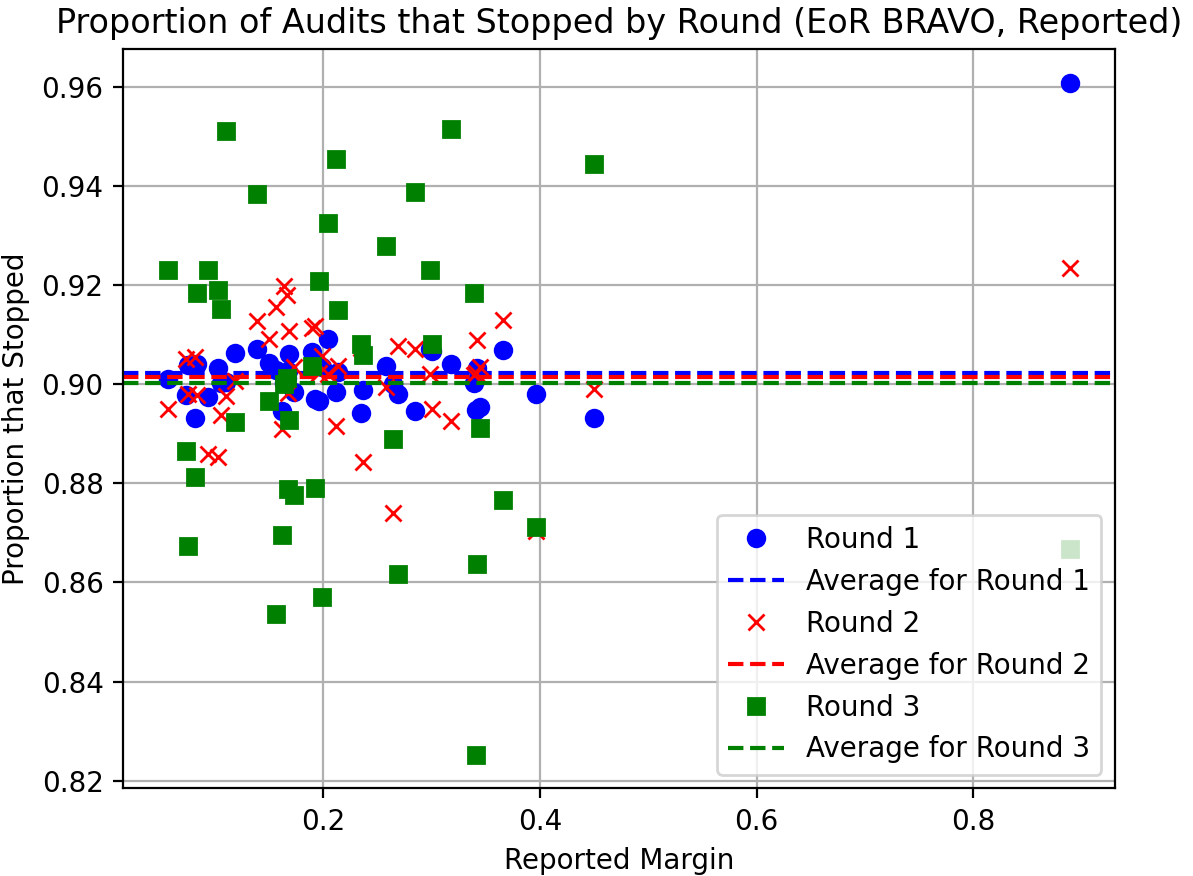
\includegraphics[width=0.8\textwidth]{eor_bravo_90perc_10^4_corrected/sprob_first_three_cropped.png}\caption{
This plot shows, for each state margin, when the underlying election is as announced, the number of EoR \BRAVO audits that stopped in the $j^{th}$ round,
as a fraction of all EoR \BRAVO audits which had not yet stopped before the $j^{th}$ round for $j=1,2,3$ and $S_1=0.9$.}
\label{fig:eor_bravo_sprob}
\end{centering}
\end{figure}

\begin{figure}
\begin{centering}
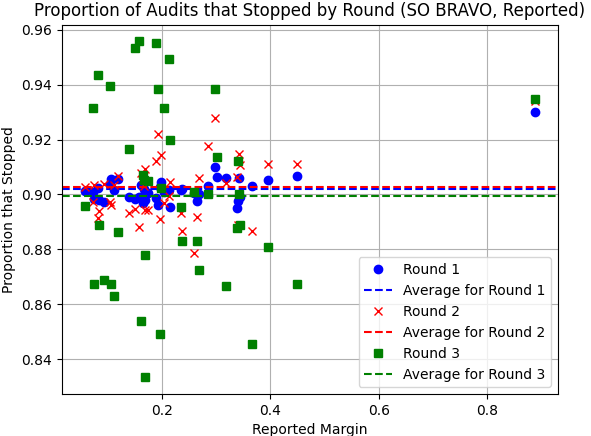
\includegraphics[width=0.8\textwidth]{so_bravo_90perc_10^4/sprob_first_three.png}\caption{
This plot shows, for each state margin, when the underlying election is as announced, the number of SO \BRAVO audits that stopped in the $j^{th}$ round,
as a fraction of all SO \BRAVO audits which had not yet stopped before the $j^{th}$ round for $j=1,2,3$ and $S_1=0.9$.}
\label{fig:so_bravo_sprob}
\end{centering}
\end{figure}

Figure~\ref{fig:minerva1_sprob} and Figure~\ref{fig:minerva1p5_sprob} show the same proportions for \Minerva round multipliers of $1.0$ and $1.5$ respectively. We see that the first round size estimates were fairly accurate, with first round stopping probabilities being very close to $.9$. For subsequent rounds, the multipliers of $1.0$ achieved smaller stopping probabilities, as it was not chosen so as to obtain $\chi_j({\mathcal A}) = 0.9$. The $1.5$ multiplier is a good estimate for $j=2$, but the stopping probability for $j=3$ is slightly smaller than $0.9$. Note that we chose a simple multiplier for future rounds, but one could make more accurate round size estimates before the audit begins. 

\begin{figure}
\begin{centering}
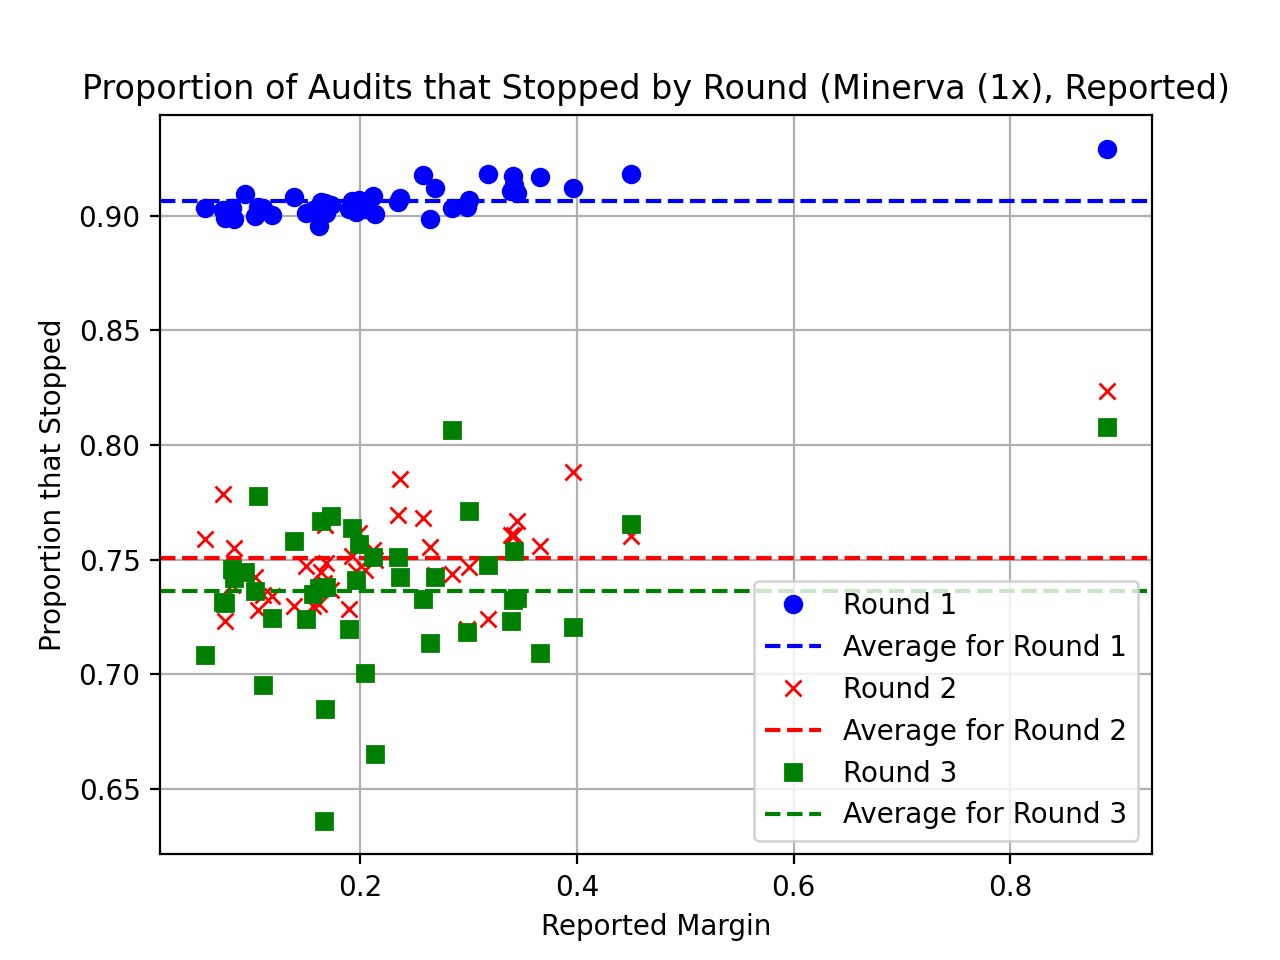
\includegraphics[width=0.8\textwidth]{minerva_multiround_1x_10^4/sprobs_first_three.png}
\caption{This plot shows, for each state margin, when the underlying election is as announced, the number of \Minerva audits that stopped in the $j^{th}$ round,
as a fraction of all \Minerva audits which had not yet stopped before the $j^{th}$ round for $j=1,2,3$, round size multiple of $1.0$ and $S_1=0.9$.}
\label{fig:minerva1_sprob}
\end{centering}
\end{figure}

\begin{figure}
\begin{centering}
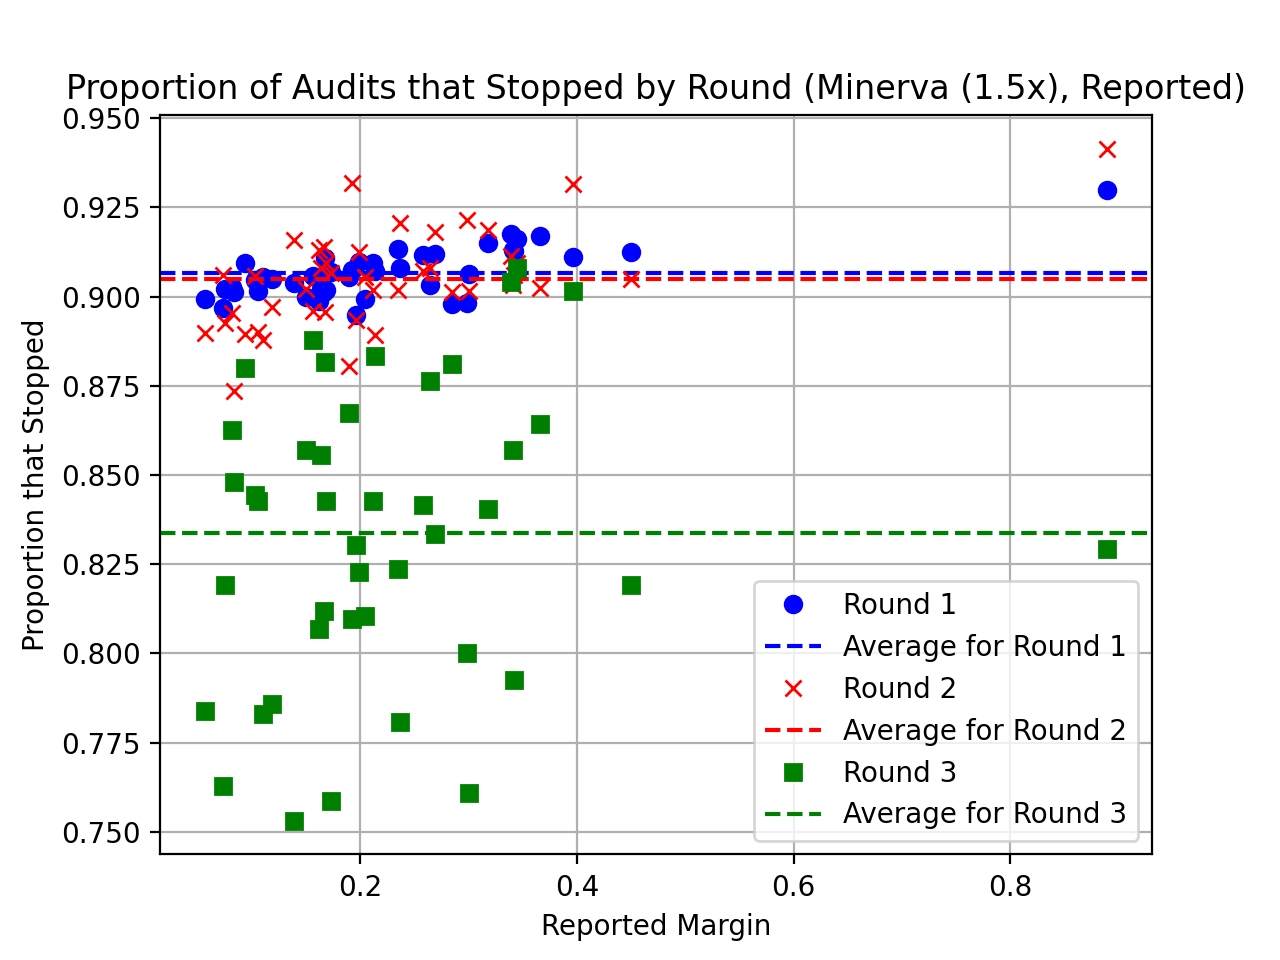
\includegraphics[width=0.8\textwidth]{minerva_multiround_1p5x_10^4/sprobs_first_three.png}
\caption{This plot shows, for each state margin, when the underlying election is as announced, the number of \Minerva audits that stopped in the $j^{th}$ round,
as a fraction of all \Minerva audits which had not yet stopped before the $j^{th}$ round for $j=1,2,3$, round size multiple of $1.5$ and $S_1=0.9$.}
\label{fig:minerva1p5_sprob}
\end{centering}
\end{figure}

Finally, we can perform a similar study for $S_1=0.25$. See Figure~\ref{fig:minerva_25} for an example, \Minerva with round mutiplier $1.5$. 

\begin{figure}
\begin{centering}
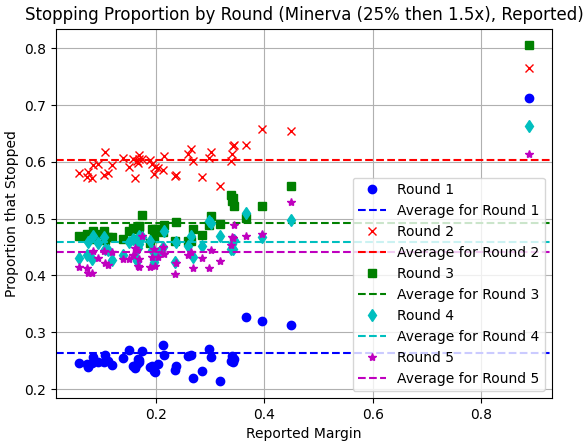
\includegraphics[width=0.8\textwidth]{minerva25percthen1p5_sprob.png}
\caption{This plot shows, for each state margin, when the underlying election is as announced, the number of \Minerva audits that stopped in the $j^{th}$ round,
as a fraction of all \Minerva audits which had not yet stopped before the $j^{th}$ round for $j=1,2,3$, round size multiple of $1.5$ and $S_1 = 0.25$.}
\label{fig:minerva_25}
\end{centering}
\end{figure}
\subsection{Maximum Risk as a Function of Round and Margin}
We also study the proportion of audits that stopped when the underlying election was a tie.
This proportion should approach a value less than the risk limit, $0.1$, as more audits are performed.

%\begin{figure}
%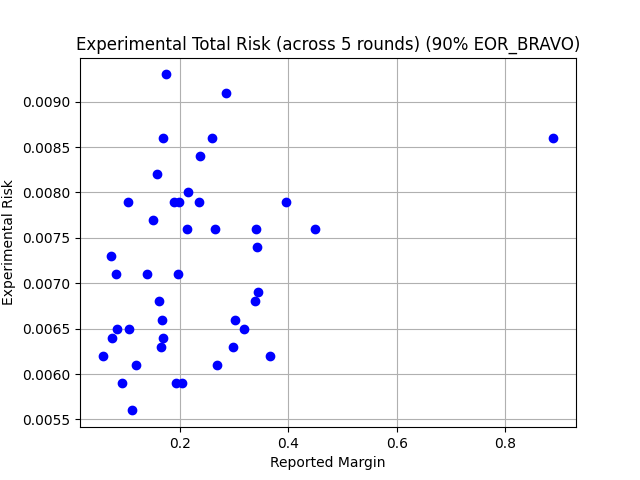
\includegraphics[width=0.8\textwidth]{eor_bravo_90perc_10^4_corrected/total_risk.png}
%\caption{This plot shows, for each state margin,
%the fraction of EoR \BRAVO audits that stopped in any of the $5$ rounds when the underlying election was a tie.}
%\label{fig:eor_bravo_risk}
%\end{figure}

\begin{figure}
\begin{centering}
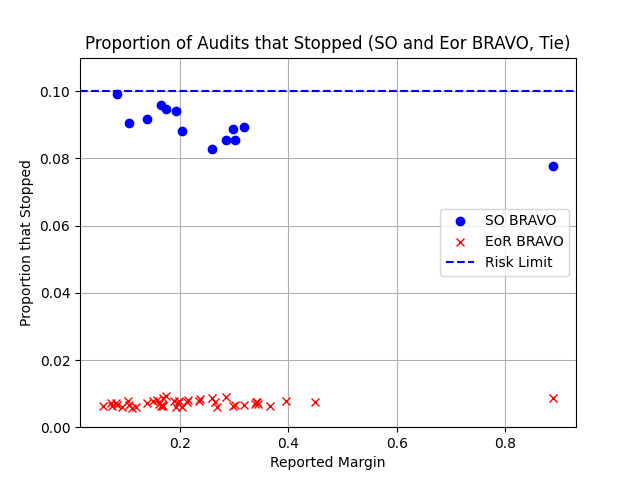
\includegraphics[width=0.6\textwidth]{bravo_risks_same_plot.png}
\caption{This plot shows the fraction of EoR \BRAVO audits (all states with margins at least $0.05$) and SO \BRAVO audits (the 13 states for which our simulations are complete so far) that stopped in any of the $5$ rounds when the underlying election was a tie.}
\label{fig:bravo_risk}
\end{centering}
\end{figure}

We observe that the risk of EoR \BRAVO is roughly
an order of magnitude less than the risk limit. 
These results are as expected, because EoR \BRAVO is known to be too conservative \cite{usenix_minerva}.  

In Figure~\ref{fig:bravo_risk} we show only the results for the $13$
states for which our simulations with an underlying tied election have completed.
To estimate the next round size that achieves a desired stopping probability,
the SO \BRAVO software generates the probability distribution on the number of ballots in the sample ballot by ballot (see \cite{usenix_minerva}) since
the stopping condition needs to be evaluated for each individual ballot drawn.
Because the underlying tied election causes audits to move on to larger rounds, 
the simulations are computationally expensive. SO \BRAVO is proven to be a Risk-Limiting Audit,
and we observe in Figure~\ref{fig:bravo_risk},
that the risk of SO \BRAVO is much
nearer the risk limit than that of EoR \BRAVO, as expected. 

%\begin{figure}
%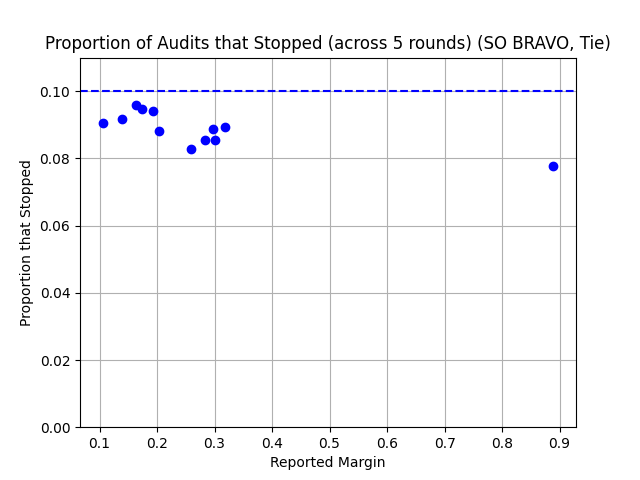
\includegraphics[width=0.8\textwidth]{so_bravo_90perc_10^4/total_risk.png}
%\caption{This plot shows, for each state margin,
%the fraction of SO \BRAVO audits that stopped in any of the $5$ rounds when the underlying election was a tie.}
%\label{fig:so_bravo_risk}
%\end{figure}

%TODO SO and EoR macros

Figure~\ref{fig:minerva1p5_risk} show that fewer than $0.1$ of the audits stopped when the underlying election was a tie, for round multiples $1.5$, as would be expected for an RLA with risk limit $0.1$. 
Unlike EOR \BRAVO, the experimental risks here are much closer to the risk limit,
showing that \Minerva stops on average with a less conservative risk; \Minerva is sharper. The plot for round multiple $1.0$ is very similar. 

%\begin{figure}
%\begin{centering}
%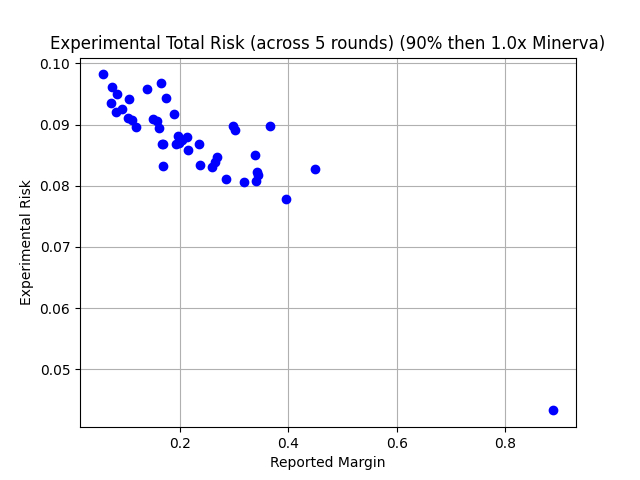
\includegraphics[width=0.6\textwidth]{minerva_multiround_1x_10^4/total_risk.png}
%\caption{This plot shows, for each state margin,
%the fraction of \Minerva audits with a round size multiple of $1.0$ that stopped in any of the $5$ rounds when the underlying election was a tie.}
%\label{fig:minerva1_risk}
%\end{centering}
%\end{figure}

%For the Minerva simulations with a round size multiple of $1.5$,
%we increased the number of simulations to $10^6$ per state for 
%both an underlying tie and underlying announced outcome. 

%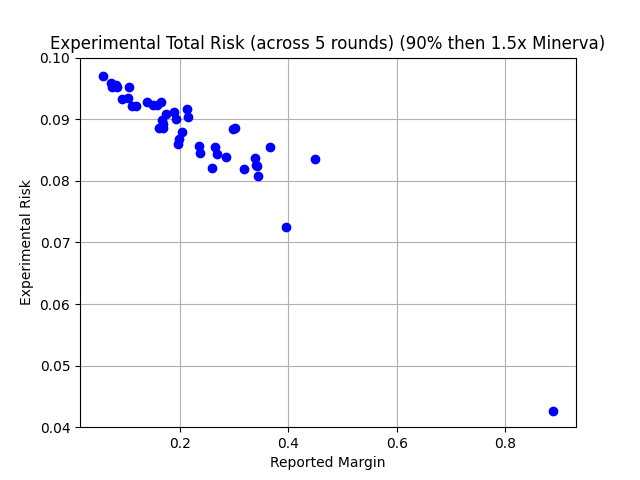
\includegraphics[width=\textwidth]{minerva_multiround_1p5x_10^6/total_risk.png}

% we could suggest that predicting accurate multiples is possible (same curve rather than line)

\begin{figure}
\begin{centering}
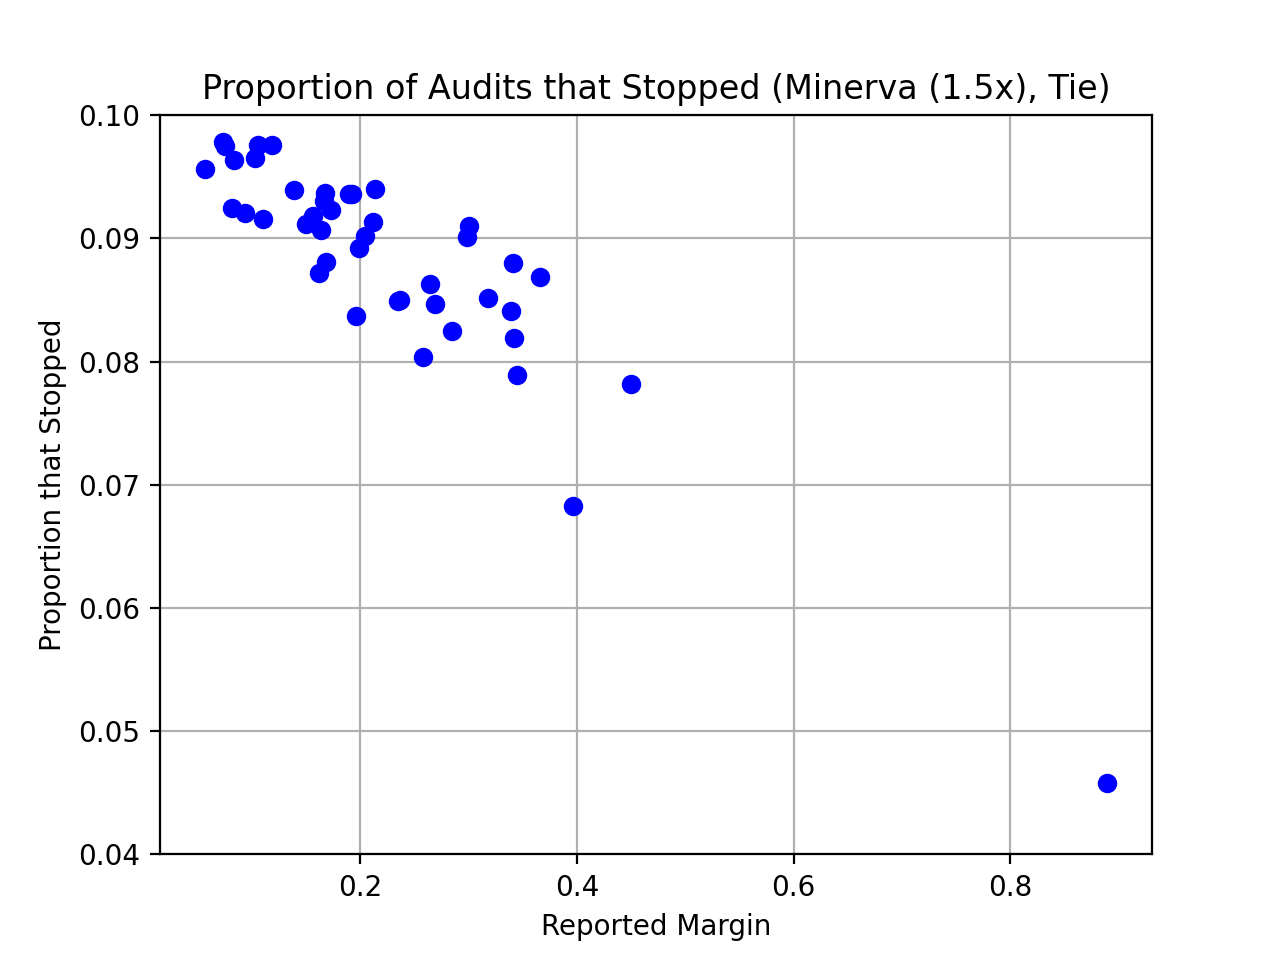
\includegraphics[width=0.6\textwidth]{minerva_multiround_1p5x_10^4/total_risk.png}
\caption{This plot shows, for each state margin,
the fraction of \Minerva audits with a round size multiple of $1.5$ that stopped in any of the $5$ rounds when the underlying election was a tie.}
\label{fig:minerva1p5_risk}
\end{centering}
\end{figure}






\section{Number of Ballots}
\label{sec:results2}
In this section we present our data on the expected number of ballots drawn as the number of rounds increases, and on the fraction of audits that stop (an estimate of cumulative stopping probability, $C_j$) for the states of Texas, Missouri and Massachusetts, with margins of $0.057$, $0.157$ and $0.342$ respectively. Interestingly, we observe that $\Minerva$ has an advantage for a first round size with stopping probability $S_1=0.25$, but it is not as large as that for $S_1=0.9$. 

\begin{figure}
\begin{centering}
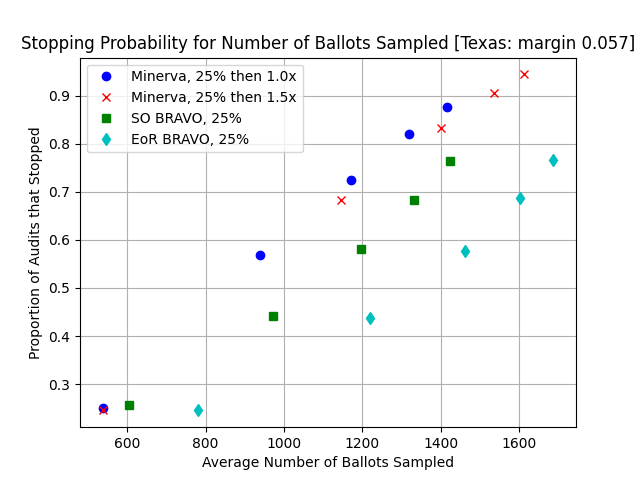
\includegraphics[width=0.75\textwidth]{texas2.png}
\caption{This plot shows the cumulative fraction of audits that stopped as a function of average number of sampled ballots for all four audits we studied, for the state of Texas, margin $0.057$, and first round stopping probability $S_1=0.25$.}
\label{fig:texas_25}
\end{centering}
\end{figure}

We observe that the behavior of both \Minerva audits is similar, and that the plot for SO \BRAVO is to the right of (more ballots) and below (lower probability of stopping) those for \Minerva, even for a stopping probability as low as $0.25$. We observe that the plot for EoR \BRAVO shows the worst performance, which is not surprising. We observe similar behavior across margins (see Figures \ref{fig:missouri_25} and \ref{fig:mass_25}), though the improvement due to \Minerva reduces as margins get larger. We see also that the improvement due to using \Minerva is not as large as that seen for $S_1=0.9$ (see Figure \ref{fig:texas_90}). 

For $S_1=0.25$, the ratio of first round size of EoR \BRAVO to \Minerva is 1.45, 1.37, 1.23 for states Texas, Missouri and Massachusetts, and margins $0.057$, $0.157$ and $0.342$ respectively. This may be compared to $2.03$, $1.99$ and $1.8$ respectively for $S_1=0.9$. 

Similarly, for $S_1=0.25$, the ratio of first round size of SO \BRAVO to \Minerva is 1.13, 1.08, 1.12 for states Texas, Missouri and Massachusetts, and margins $0.057$, $0.157$ and $0.342$ respectively. This may be compared to $1.38$, $1.38$ and $1.30$ respectively for $S_1=0.9$. 

\begin{figure}
\begin{centering}
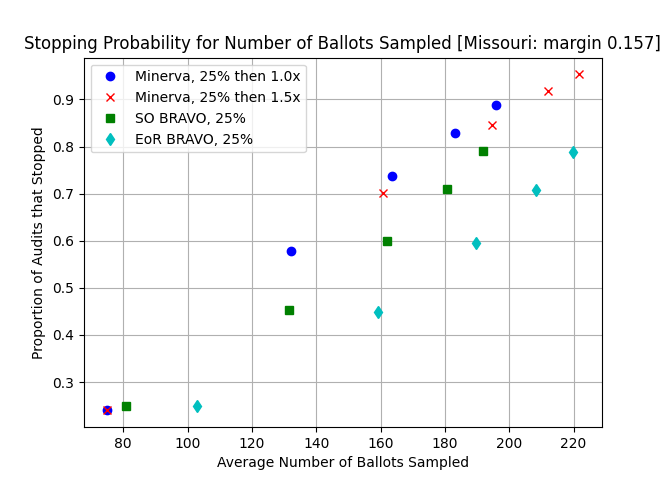
\includegraphics[width=0.75\textwidth]{missouri2.png}
\caption{This plot shows the cumulative fraction of audits that stopped as a function of average number of sampled ballots for all four audits we studied, for the state of Missouri, margin $0.157$, and first round stopping probability $S_1=0.25$.}
\label{fig:missouri_25}
\end{centering}
\end{figure}

\begin{figure}
\begin{centering}
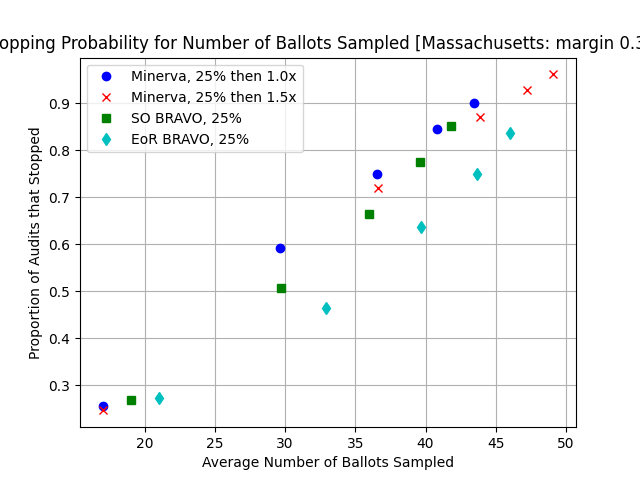
\includegraphics[width=0.75\textwidth]{massachusetts2.png}
\caption{This plot shows the cumulative fraction of audits that stopped as a function of average number of sampled ballots for all four audits we studied, for the state of Massachusetts, margin $0.342$, and first round stopping probability $S_1=0.25$.}
\label{fig:mass_25}
\end{centering}
\end{figure}

\begin{figure}
\begin{centering}
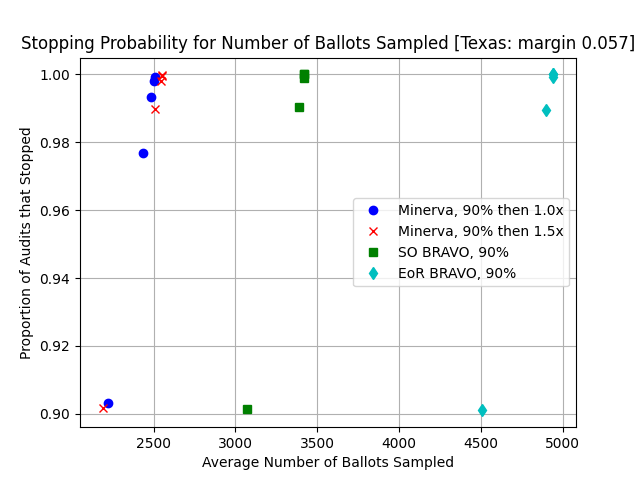
\includegraphics[width=0.75\textwidth]{texas1.png}
\caption{This plot shows the cumulative fraction of audits that stopped as a function of average number of sampled ballots for all four audits we studied, for the state of Texas, margin $0.057$, and first round stopping probability $S_1=0.9$.}
\label{fig:texas_90}
\end{centering}
\end{figure}



\section{Conclusions and Future Work}
\label{sec:conc}
%Conclusions

%\section{Acknowledgements}
%\label{sec:ack}
%This research was supported in part by NSF Awards 2015253
%and 1421373.


%
% ---- Bibliography ----
%
% BibTeX users should specify bibliography style 'splncs04'.
% References will then be sorted and formatted in the correct style.
%
\bibliographystyle{splncs04}
\bibliography{audits}
%
\end{document}

